\begin{tcolorbox}
\chapter{2009 - Brezzvezdna Noč}

The 2009 Brezzvezdna Noč expedition was extremely successful, with 4
weeks spent in the field camping by special permission in the Triglav
national park on \passage{Tolminski Migovec}. 

During the 2008 expedition a considerable effort was spent exploring the
\passage{Captain Kangaroo} branch of \passage{Vrtnarija}, with the sole aim of
connection to the passage in \passage{Sistem Migovec}. Our rate of exploration was
limited by the length of time taken to get to the pushing front, with
fifteen hour trips being the minimum to achieve much. The obvious
solution for 2009 was to set up a camp.

A literal translation of Brezzvezdna Noč from Slovene is 'Starless Night', and emphasises the underground camping focus of this expedition, in the context of ICCC's extremely productive and long term partnership with the JSPDT. Pronunciation for English is fairly close to Brezz-vezzd-na Notch.

\end{tcolorbox}
\backgroundsetup{
    scale=1,
    color=black,
    opacity=1,
    angle=0,
    contents={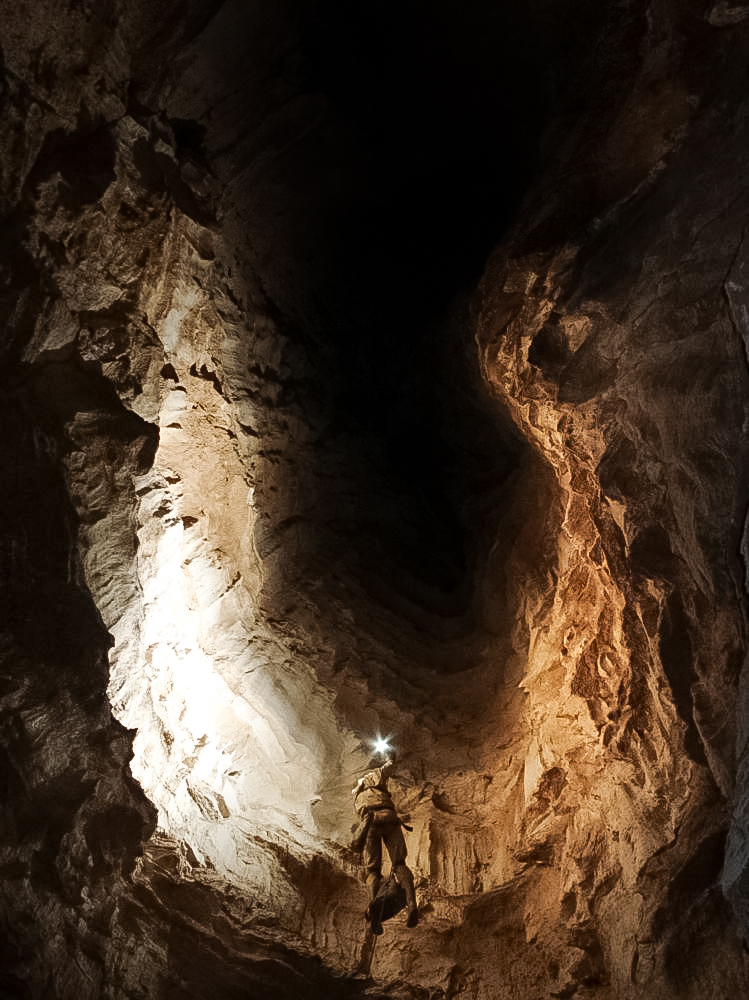
\includegraphics[height=\paperheight]{2009/intro/2009-08-10-18.25.30 - Jarvist Frost - Canon Powershot G5 - dark tranquility - gergely 10 odd metres from ground single vivitar 283 flash--orig.jpg}}
}
\BgThispage









